\vspace{15px}

Un SoC est composé de blocs correspondant chacun à un module spécifique (CPU, interfaces RS232, USB, PCI, modules de traitement du signal, blocs réseaux ARM ou Ethernet, module d'encryption DES ou AES ...). Heureusement il n'est pas à chaque fois nécessaire de tout réadapter. La plupart des modules écrit pour un certain projet sont réutilisables dans d'autres, ils ont été souvent prévus pour une intégration plug and play. Chacun des blocs constitue un bloc Soft-IP (Soft Intellectual Property Block) en opposition aux Hard-IP Blocks (ASIC), généralement bien documenté afin de faciliter le travail de réintégration et dont la licence encadre ses conditions de réutilisation au sein d'un projet (licence propriétaire entrainant le paiement de droit ou licences opensources avec chacune leurs partucalarités). Les avantages de blocs IP sont nombreux, ils permettent de supprimer le temps d'écriture du bloc donc diminuer le temps jusqu'à la commercialisation, diminuer le nombre d'ingénieurs requis pour le projet donc diminuation des coûts  et enfin rassurer les développeurs car la solution est déjà prouvée.
\medskip

\begin{center}
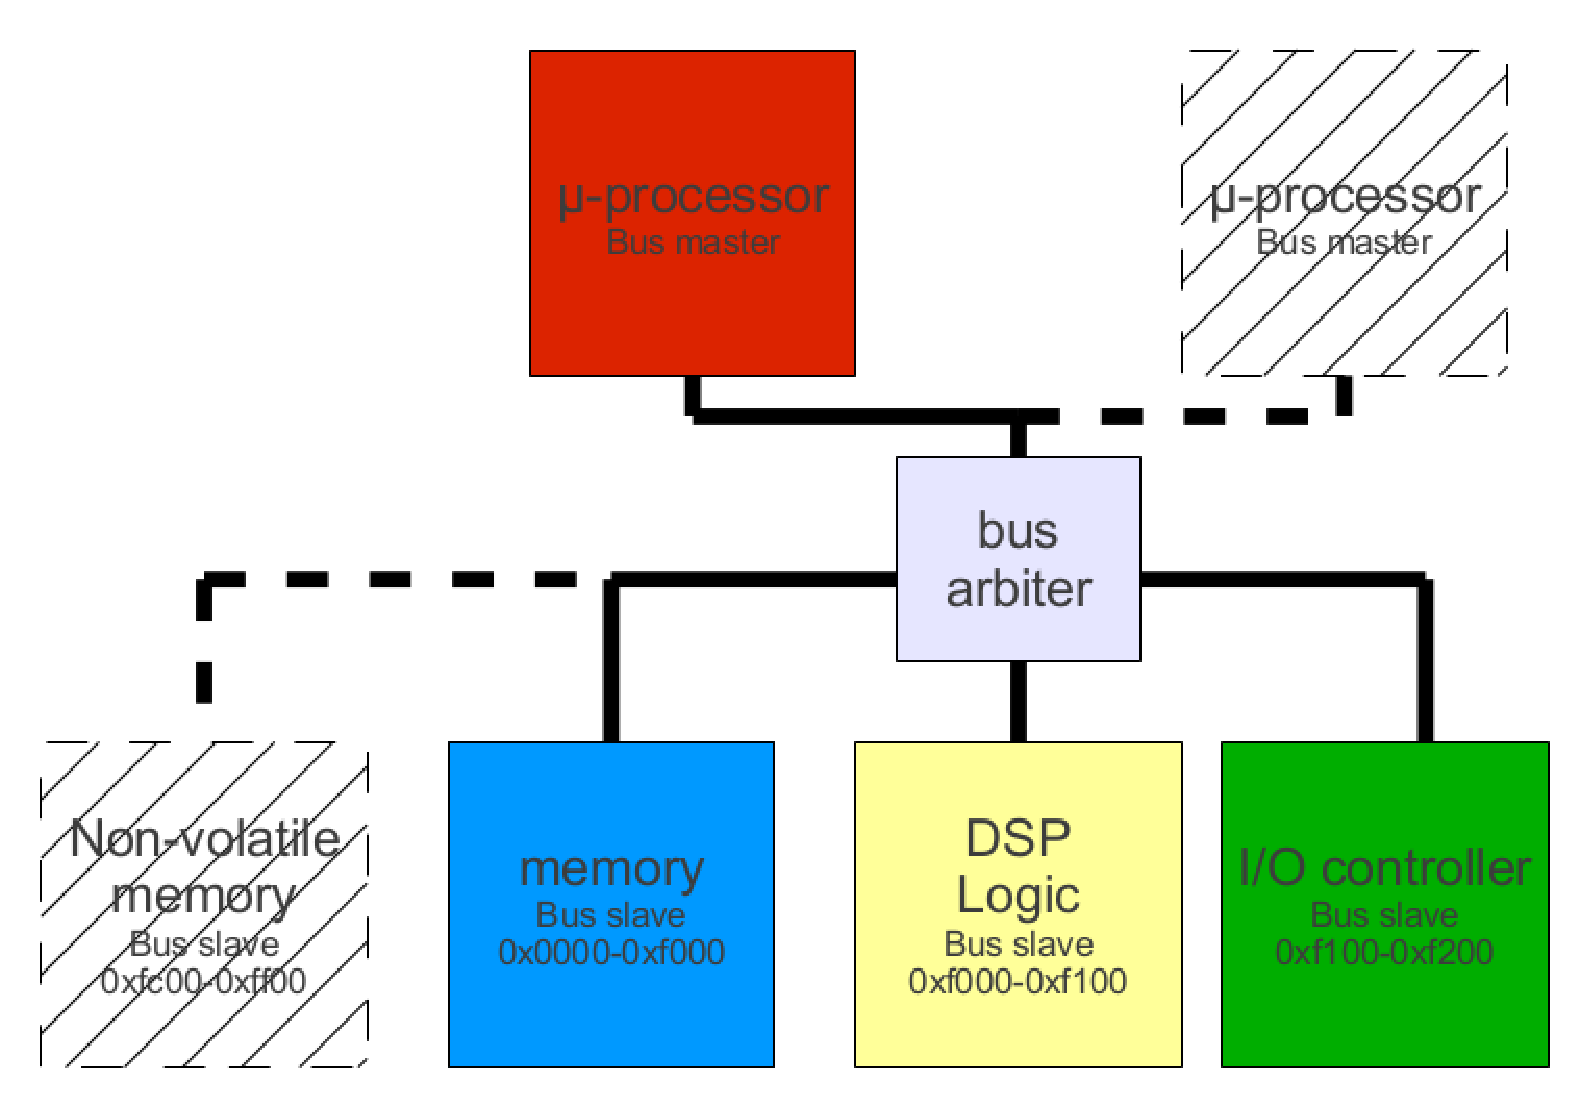
\includegraphics[scale=0.4]{soc_arch.eps}
\end{center}

Seule la description du circuit (les interconnections entre les différents modules et les entrées/sorties du FPGA) est écrite à chaque fois que l'on change de carte ou/et de FPGA. Cette description peut être codée soit en VHDL ou en Verilog tout comme la description des blocs. Il s'agit souvent d'un memory-mapped bus fournissant un accès aux registres de contrôle et aux mémoires. Dans notre cas, c'est un CSR bus conçu par Sébastien Bourdeauducq, à l'origine du projet MilkyMist.
\medskip

\begin{center}
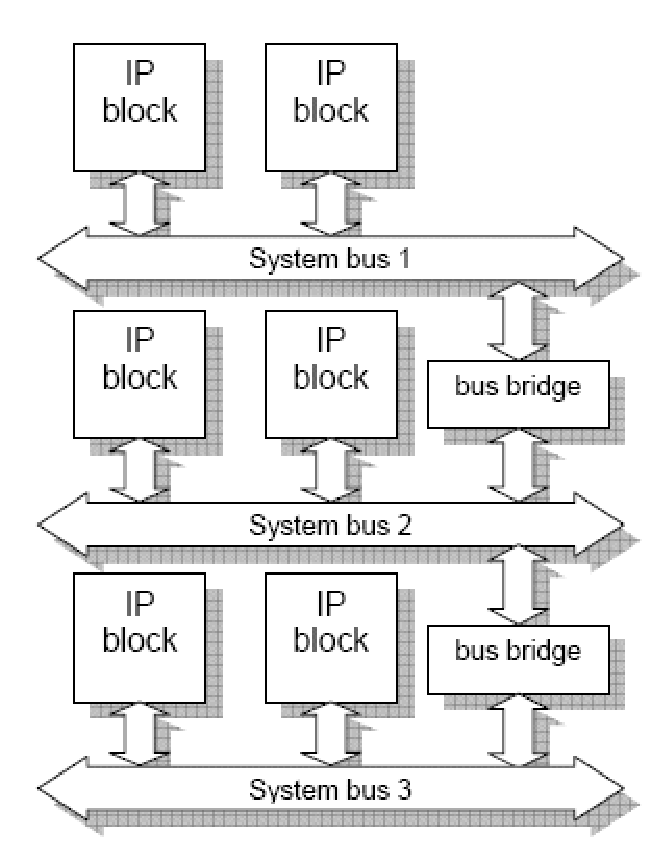
\includegraphics[scale=0.4]{soc_interconnect.eps}
\end{center}

Dans notre cas, nous allons réutiliser plusieurs modules déjà implémentés. Tout d'abord, l'IP-Core LatticeMico32 (architecture RISC) déjà intégré dans MilkyMist et disponible gratuitement sous licence GNU GPL. Celui ci nécessite tout de même dû à sa généricité quelques configurations lorsqu'on le change de FPGA (taille du bus, nombre de registres, alimentation, timing, taille du cache, …) et on peut également choisir selon ses besoins d'implémenter ou non afin d'économiser des portes logiques certaines parties dans l'unité de calcul (unité de multiplication, de décalage, activer les calculs signés, ...).
\medskip

Va être aussi réutilisé le GPIO, l'USART, la ROM qui contiendra le BIOS, … (à revoir cette partie là, y'a tellement de truc commenté et décommenté dans le fichier que c'est resté flou dans ma tête).
\medskip

Chacun d'eux va être configuré tout comme le processeur selon nos besoins.
\medskip

Dans cette partie, nous avons vu l'énorme utilité de la généricité dans la description des IPs. Cet espect est souvent utilisé dans l'industrie afin de créer un hardware spécifique à nos besoins. On peut gagner par cette méthode énormément en efficacité face aux architectures non-spécialisées, ce qui permet pour un résultat égal de travailler à fréquence plus basse et du coup de moins chauffer et consommer d'énergie.
\medskip